\documentclass[a4paper,11pt]{article}
\usepackage[utf8]{inputenc}
%\usepackage[spanish]{babel}
\usepackage{amsmath, amssymb}
\usepackage{graphics, subfigure}
\usepackage{lipsum}
\usepackage{array}
\usepackage{url}
\usepackage[top=2.5cm, bottom=2.5cm, left=2cm, right=2cm]{geometry}
\usepackage{float}
\usepackage{multicol}
\usepackage{enumerate}
\usepackage{color, xcolor}
\usepackage{fancyvrb}
\usepackage[hidelinks]{hyperref}
\usepackage{graphicx}
\usepackage{multicol}
\usepackage{listings}
\usepackage{color}

\begin{document}

\begin{center}
\begin{Large}
\rule{\textwidth}{0.5pt}
\par Universidad de la Habana, MATCOM
\par Programación Declarativa (2021)
\vspace{0.4cm}
\par \textcolor{cyan}{Juego Hive}
\end{Large}

\vspace{1mm}
\par Samuel David Suárez Rodríguez C412
\par Enmanuel Verdesia Suárez C411
\rule{\textwidth}{1.5pt}
\end{center}

\vspace{0.5cm}

\lstset{frame=tb,
  language=Prolog,
  aboveskip=3mm,
  belowskip=3mm,
  showstringspaces=false,
  columns=flexible,
  basicstyle={\small\ttfamily},
  numberstyle=\tiny\color{gray},
  keywordstyle=\color{blue},
  commentstyle=\color{dkgreen},
  stringstyle=\color{mauve},
  breaklines=true,
  breakatwhitespace=true,
  tabsize=3
}

\definecolor{dkgreen}{rgb}{0,0.6,0}
\definecolor{gray}{rgb}{0.5,0.5,0.5}
\definecolor{mauve}{rgb}{0.58,0,0.82}

\section{Detalles de Implementación}

El juego fue creado usando \verb+SWI-Prolog 8.2.4+. En dicho lenguaje se implementó toda la lógica para la ejecución de la Inteligencia Artificial (IA).

\subsection{Sistema de Coordenadas}

Se empleó un sistema axial de coordenadas para representar la posición de las piezas en el tablero, donde la posición de cada pieza está determinada por dos componentes $(q, r)$ como se muestra en la imagen a continuación.

\begin{figure}[H]
\centering
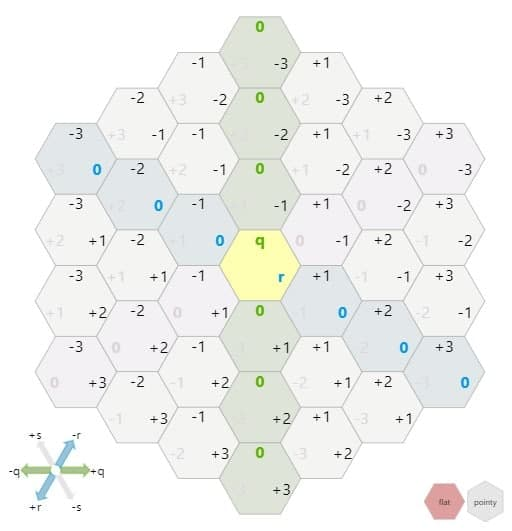
\includegraphics[width=0.3\textwidth]{images/hex_grid.jpg}
\caption{Cuadrícula hexagonal.}
\end{figure}

\subsection{Estados}

Para representar una pieza se usó un predicado de la siguiente forma:

\verb+piece(Class, Color, Id, Q, R, S).+

\begin{itemize}
\item[•] \verb+Class+: es el tipo de la pieza dentro del juego de Hive: reina (\verb+'q'+), saltamontes (\verb+'g'+), araña (\verb+'s'+), mariquita (\verb+'l'+), hormiga (\verb+'a'+), escarabajo (\verb+'b'+) o mosquito (\verb+'m'+).

\item[•] \verb+Color+: el color del jugador a quien corresponde la pieza (\verb+'b'+ o \verb+'w'+).

\item[•] \verb+Id+: el identificador de la cada pieza para diferenciarla de otras con la misma clase.

\item[•] \verb+Q+ y \verb+R+: las componentes correspondientes en el sistema de coordenadas.

\item[•] \verb+S+: \'indice de apilaci\'on que tiene la pieza en caso de estar encima de otra.
\end{itemize}

Estos predicados son almacenados en la Base de Datos (BD) local de Prolog, manteniendo así el estado actual del sistema. Por tanto modificar el estado implica agregar y/o eliminar predicados en la BD. Mediante el siguiente predicado se consulta dicho estado.

\verb+get_pieces(Pieces) :-+

\verb+  findall(+

\verb+    piece(Class, Color, Id, Q, R, Stacked),+

\verb+    piece(Class, Color, Id, Q, R, Stacked),+

\verb+    Pieces+

\verb+  ).+

\subsection{Consistencia de la Colmena}

En todo momento se mantiene la consistencia de la colmena, de tal forma que esta no se divida en una o más partes motivo del movimiento de una pieza a una nueva posición. Por tanto si una pieza es punto de articulación (eliminarlo causaría que el grafo formado por las piezas deje de ser conexo) esta no puede ser movida a otra posición hasta que deje de serlo. El predicado a continuación realiza dicha validación.

\begin{lstlisting}
articulation_point(piece(Class, Color, Id, Q, R, S)) :-
  get_pieces(Pieces),
  length(Pieces, LPieces),
  Remaining is LPieces - 1,
  piece_neighbours(Q, R, [Start|_]),
  remove_piece(piece(Class, Color, Id, Q, R, S)),
  connected_component([Start], [], Component),
  add_piece(piece(Class, Color, Id, Q, R, S)),
  length(Component, LComponent),
  Remaining \= LComponent.
 
connected_component([], Marked, Component) :- append([], Marked, Component).
connected_component([piece(Class, Color, Id, Q, R, S) | Stack], Marked, Component) :-
  piece_neighbours(Q, R, Neighbours),
  member(Next, Neighbours),
  \+ member(Next, Marked),
  append(Stack, [Next], NStack),
  append(Marked, [Next], NMarked),
  connected_component([piece(Class, Color, Id, Q, R, S) | NStack], NMarked, Component), !.
connected_component([_ | Stack], Marked, Component) :-
  connected_component(Stack, Marked, Component).
\end{lstlisting}

Donde \verb+piece_neighbours+ es un predicado que dada la posición de una pieza obtiene todas la piezas que son adyacentes a esta y \verb+connected_component+ devuelve la lista de elementos en una componente conexa comenzando en alguna pieza. Si al eliminar la pieza y llamar \verb+connected_component+ obtenemos menos de la cantidad de piezas que restan en el tablero, podemos decir que es un punto de articulaci\'on y por tanto rompe la colmena.

\subsection{Transiciones de estados}

Un juego no es más que una lista de acciones secuenciales que van modificando los estados, en nuestro caso una acci\'on se representa como

\begin{lstlisting}
action(
  Piece1,
  Piece2,
  Side
)
\end{lstlisting}

En donde \verb+Piece1+ y \verb+Piece2+ son piezas y \verb+Side+ puede tomar uno de estos posibles valores:

\begin{itemize}
\item[•] \verb+N+ (Al norte de)

\item[•] \verb+NW+ (Al noroeste de)

\item[•] \verb+SW+ (Al suroeste de)

\item[•] \verb+NE+ (Al noreste de)

\item[•] \verb+SE+ (Al sureste de)

\item[•] \verb+S+ (Al sur de)

\item[•] \verb+O+ (Sobre)
\end{itemize}

Esto indica la posici\'on donde colocar la pieza \verb+Piece1+ respecto a \verb+Piece2+.

Un ejemplo de acci\'on puede ser

\begin{lstlisting}
action(
  piece(a, b, 3, 1, -3, 0),
  piece(q, w, 1, 0, 1, 0),
  NW
)
\end{lstlisting}

que se traduce como

\begin{flushleft}
\verb+'La hormiga negra con id 3 se posiciona al noroeste de la reina+
\verb+blanca con id 1.'+
\end{flushleft}

Los edge cases aqu\'i son  los movimientos de adici\'on de una pieza al tablero y la primera acci\'on del juego que tambi\'en es de adici\'on pero sin ninguna pieza respectiva, cuando esto pasa decidimos por convenio igualar los valores de \verb+Piece1+ y \verb+Piece2+, sin importar el valor de \verb+Side+, y para el segundo edge case hacemos una diferenciaci\'on si nos encontramos en el turno 1.

Como detalle cabe aclarar que si una pieza no se encuentra en el tablero actualmente entonces los valores de su posici\'on \verb+Q, R, S+ son -1. Esta es una posici\'on v\'alida si solo tenemos en cuenta \verb+Q, R+, sin embargo como \verb+S+ debe ser mayor o igual que cero nos sirve para diferenciar los casos.

Con respecto a la implementaci\'on, definimos un predicado \verb+step+ que recibe una acci\'on y un turno y en caso de que la acci\'on sea correcta, actualiza el estado actual. Para las validaciones implementamos predicados especificos para cada tipo de pieza, en el que cada tipo tiene un predicado \verb+<tipo>_can_move+ que recibe la pieza y una posici\'on y chequea si esa pieza se puede mover. De esta manera, en caso de que la acci\'on sea de movimiento, llamamos al predicado correspondiente seg\'un la pieza que se quiera mover en la acci\'on, y si el resultado triunfa, movemos la pieza. En caso de la adici\'on las validaciones son las mismas para cualquier tipo de pieza, por lo que implementamos un predicado que lo valide.

Este tipo de organizaci\'on en el c\'odigo para validar las acciones nos permite de una manera limpia validar especialmente el movimiento del mosquito,
cuya validaci\'on cambia en dependencia de las piezas adyacentes, el c\'odigo
para esto es el siguiente

\begin{lstlisting}
mosquito_can_move(piece(Class, Color, Id, Q, R, S), position(NQ, NR, NS), C) :-
  (C = q, queen_can_move(piece(Class, Color, Id, Q, R, S), position(NQ, NR, NS)));
  (C = a, ant_can_move(piece(Class, Color, Id, Q, R, S), position(NQ, NR, NS)));
  (C = l, ladybug_can_move(piece(Class, Color, Id, Q, R, S), position(NQ, NR, NS)));
  (C = s, spider_can_move(piece(Class, Color, Id, Q, R, S), position(NQ, NR, NS)));
  (C = g, grasshopper_can_move(piece(Class, Color, Id, Q, R, S), position(NQ, NR, NS)));
  (C = b, beetle_can_move(piece(Class, Color, Id, Q, R, S), position(NQ, NR, NS))).

mosquito_can_move(piece(Class, Color, Id, Q, R, S), position(NQ, NR, NS)) :-
  piece_neighbours(Q, R, Neighbours),
  member(piece(NeighbourClass, _, _, _, _, _), Neighbours),
  mosquito_can_move(piece(Class, Color, Id, Q, R, S), position(NQ, NR, NS), NeighbourClass).
\end{lstlisting}

por lo que un mosquito puede moverse a una posici\'on cuando posee un vecino tal que alguno de los predicados anteriores triunfe.

\subsection{Interacci\'on con el usuario}

Para iniciar el juego se debe llamar el archivo \verb+main.pl+, ejecutar \verb+main().+ y seguir las instrucciones.

El usuario interact\'ua en el juego escribiendo de una manera codificada la acci\'on que quiere realizar, por ejemplo

\verb+ba3 NW wq1+

corresponde a la acci\'on descrita anteriormente donde la hormiga negra se mueve al noroeste de la reina blanca. El primer caracter de cada pieza indica el color, luego el tipo de pieza seguido por el id, y en el medio y separado por espacios se indica el valor de \verb+Side+. En caso de la primera jugada
solo se escribir\'a la pieza que se quiere colocar, por ejemplo

\verb+wq1+

En cada momento luego de realizar una acci\'on se devuelve en forma de lista los valores de cada \verb+piece+ que hay en el tablero, de esa manera sabremos el estado actual, en caso de que la jugada sea inv\'alida se le notificar\'a al usuario un mensaje con la descripci\'on del error que cometi\'o.

\subsection{Inteligencia artificial}

El juego posee una variante \verb+pve (Player vs Environment)+ en el que el usuario puede jugar contra un agente. Este agente implementa una heur\'istica sencilla basada en asignarle valores a cada estado y en cada turno observar qué acci\'on maximiza el valor del siguiente estado.

La funci\'on de estado se califica de la manera siguiente

\begin{itemize}
\item[•] Si el estado es ganador, asignamos un valor lo suficientemente grande para ser mayor que los dem\'as estados (500), puesto que llegar a este estado implica una victoria.

\item[•] Si el estado es una derrota, asignamos el menor valor posible (-500), puesto que es el estado que queremos evitar.

\item[•] Si el estado es un empate, asignamos el valor 5. En un principio podemos pensar en asignar el valor medio de los estados ganadores y perdedores (250), sin embargo esto conlleva a que nuestro agente priorize empatar que realizar otras acciones que pueden llevarlo a ganar, por eso le dimos menos prioridad a los empates.

\item[•] En cualquier otro caso calculamos el valor de un estado con la siguiente f\'ormula.

\begin{lstlisting}
	10 * (OponentPiecesAroundQueen - PlayerPiecesAroundQueen)
    + 2 * (LengthPlayerFreePieces - LengthOponentFreePieces)
    + (LengthPlayerPiecesOnBoard - LengthOponentPiecesOnBoard)
\end{lstlisting}

es una suma de t\'erminos donde indicamos a qu\'e detalles del estado le damos prioridad. El primer t\'ermino es la diferencia entre la cantidad de piezas que rodean a la reina del oponente menos las del agente, es el t\'ermino con m\'as prioridad, y que hace que el agente rodee la reina enemiga y mueva su reina cuando tiene muchos vecinos que la bloquean. El segundo t\'ermino mide la diferencia entre la cantidad de piezas que no estan rodeadas en el tablero entre el agente y el oponente, lo que prioriza tener una mayor libertad entre las piezas en el tablero. Por \'ultimo el tercer t\'ermino es la diferencia entre la cantidad de piezas entre el agente y el oponente, lo que permite agregar piezas en el tablero en el early game, luego esta decisi\'on va perdiendo prioridad debido a que los otros casos aportan mayor valor, pero permiten una mayor flexibilidad en los primeros turnos.
\end{itemize}

Este agente encapsula todo el algoritmo en un predicado \verb+choose_action(Color, Action, Turn)+ que decide cu\'al acci\'on realizar dado el estado actual, para probar cada acci\'on llamamos la funci\'on \verb+step+ de la que hablamos anteriormente, y tambi\'en definimos un predicado \verb+undo_action+ que revierte la acci\'on realizada, este predicado es usado exclusivamente por el agente.

\section{C\'odigo fuente}

\verb+https://github.com/Team-Secrett/hive/+

\end{document}
